\section{Appendix}
\subsection{Survey Structure}
Our survey consists of two types of questions. We ask participants to either evaluate statements we make about the European debt crisis or ask to which party a certain statement applies. We further ask participants regarding their knowledge about the European debt crisis and socioeconomic characteristics. Our survey is structured in the following way. Our first question consists of asking people whether a country from the Eurozone received financial assistance. Participants can choose between three options: Yes, No and I don't know. Our second question asks about the beginning of the financial rescue program. 
Participants can indicate whether they strongly agree, slightly agree, slightly disagree or strongly disagree with or don't know about the following statements. 
The lender countries wanted to help the borrower countries. The lender countries wanted to help avoid a crisis at home. The lender countries wanted to impose institutional change upon the borrower countries. 
In the third question participants are asked "Who was the driving force behind the rescue program". In the fourth question they are asked "Which party benefited most from the rescue program" for both questions participants have the answer options: The lender countries, both parties equally, the borrower countries and I don' know. In the fifth question participants are asked about the feelings the rescue program evoked among the citizens from the borrower countries and the lender countries. As with question two participants have the option to answer with strongly agree, slightly agree, slightly disagree and strongly disagree or the option I don't know. The statements participants are asked to assess are the following: The rescue experience made citizens from the borrower countries feel guilty, the rescue experience made citizens from the borrower countries feel exploited, the rescue experience made citizens from borrower countries feel inferior, the rescue experience made citizens from lender countries feel exploited, rescue experience made citizens from the lender countries feel disappointed and the rescue experience strengthened friendships. In the last two questions of the survey participants are asked about the situation in Greece. The sixth question of our survey asks participants which party benefited most from loans to Greece. The answer options include Greece, the lender countries, both equally and I don't know. The last question of our survey asks participants whether Greece will repay it's debt. Participants can answer strongly agree, slightly agree, slightly disagree, strongly disagree and I don't know. Participants from both samples are asked the same questions. However, participants of the World Economic Survey are interviewed on a regular basis. Their survey further included questions on other macroeconomic variables. The survey was distributed to the participants on paper, while the participants recruited through the website prolific answered the survey online. In a comparison of the results from online and pen-and paper survey outcomes \cite{abel} finds no differences in the responses of participants. 


\subsection{Heterogeneity Analysis}
\textbf{Socioeconomic Characteristics}

\begin{figure} [h!]
    \begin{center}
     \caption{ Intentions of the borrower countries}
    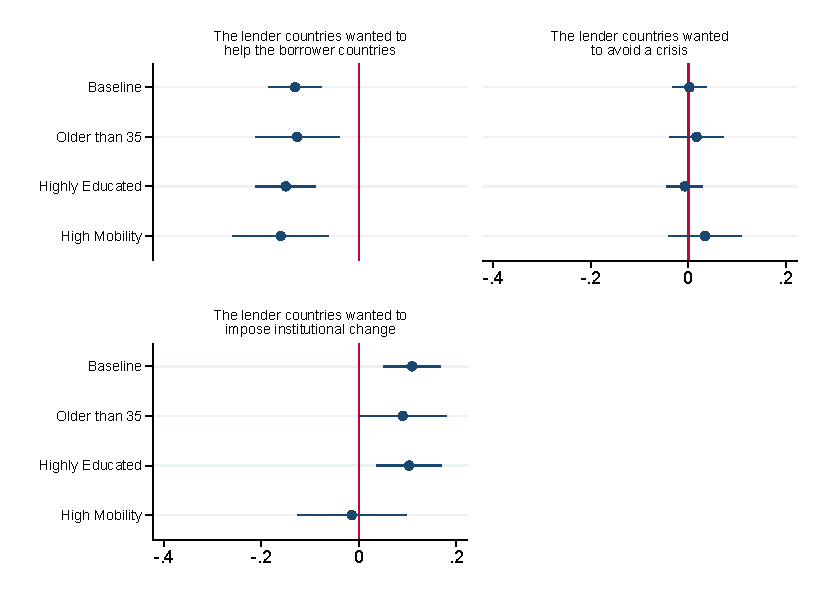
\includegraphics[scale=1.2]{socio_question2.pdf}
    \label{fig:my_label}
    \end{center}
    \tiny 
    \tablenotes{Participants were asked to assess the following statements:  Question 2.1: The lender countries wanted to help the borrowing countries Question 2.2: The lender countries wanted to help themselves avoid a crisis at home Question 2.3: The lender countries wanted to impose institutional change upon the borrower countries }
\end{figure}
\begin{figure}[h!]
    \begin{center}
     \caption{ Emotions of program countries}
    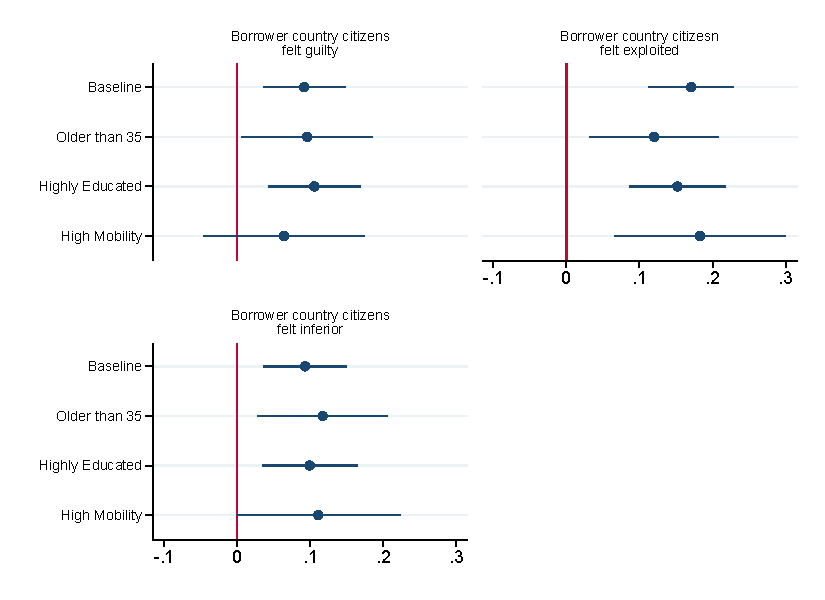
\includegraphics[scale=1.2]{socio_question5_1.pdf}
    \label{fig:my_label}
    \end{center}
    \tiny 
     \tablenotes{Question 5.1: The rescue experience made many citizens in the borrower countries feel guilty; Question 5.2: The rescue experience made many citizens in the borrower countries feel exploited; Question 5.3: The rescue experience made many citizens in the borrower countries feel inferior} 
\end{figure}
\begin{figure}[h!]
    \begin{center}
     \caption{ Emotions of non-program countries and repayment of outstanding debt}
    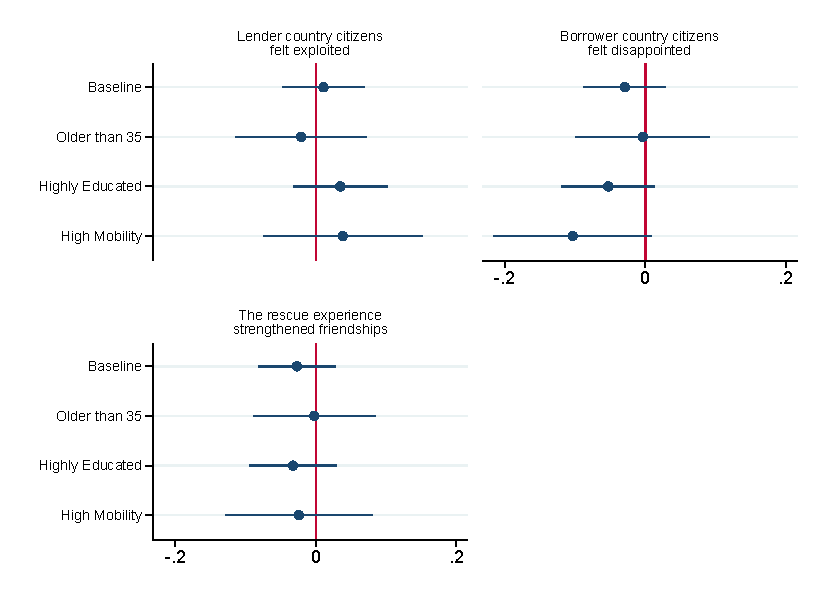
\includegraphics[scale=1.2]{socio_question5_2.pdf}
    \end{center}
    \tiny
     \tablenotes{Question 5.4: The rescue experience made many citizens in the lender countries feel exploited; Question 5.5 The rescue experience made many citizens in the lender countries feel disappointed Question 5.6: The rescue experience strengthened friendships between citizens Question 7: Greece will fully pay back it's debt}
\end{figure}
\begin{figure}[h!]
    \begin{center}
     \caption{Who initiated and benefited from the rescue program}
    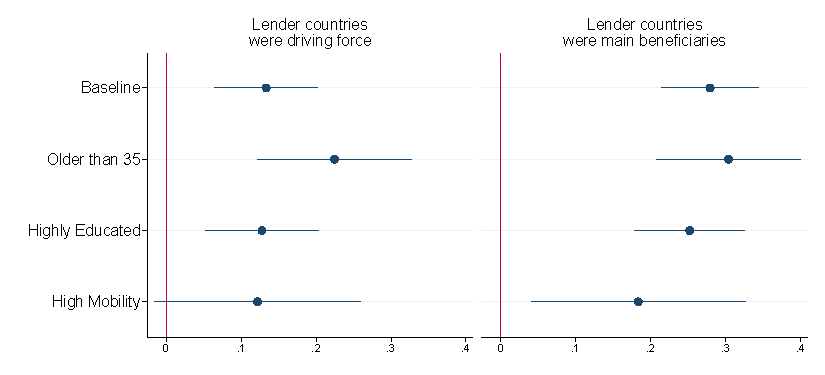
\includegraphics[scale=0.9]{socio_question3_4.pdf}
    \end{center}
    \tiny
    \tablenotes{Question 3: Who was the driving force behind signing the memorandum; Question 4: Who was the main beneficiary of the program; Question 7: Who primarily benefited from the loans to Greece}
\end{figure}
\begin{figure}[h!]
    \begin{center}
     \caption{Situation in Greece}
    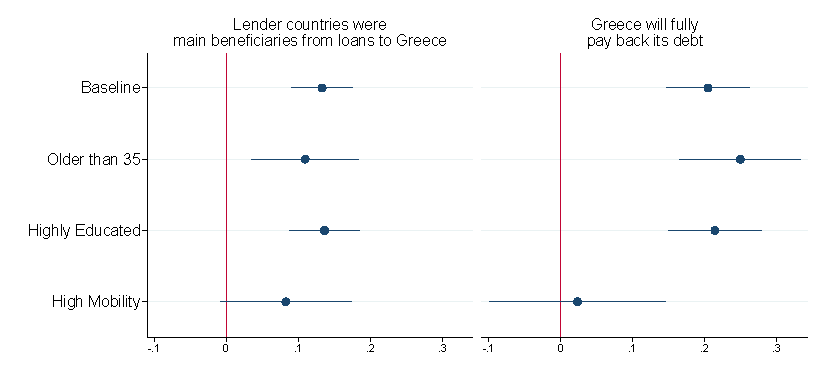
\includegraphics[scale=0.9]{socio_question6_7.pdf}
    \end{center}
    \tiny
    \tablenotes{Question 6: Who primarily benefited from the loans to Greece? ;  Question 7: Greece will fully pay back it's debt}
\end{figure}
\clearpage


\textbf{Knowledge and Beliefs}
%articipants differ in their level of knowledge about the European debt crisis. Some people fail to correctly identify their country as a borrower or lender country. An overview of the fraction of participants who knew their country's status can be found in the appendix. However, knowledge about the status of one's country does not appear to influence the observed effects. The estimates of the baseline model on the subsample of non-experts who could correctly identify their country does not change in comparison to the estimates for the full sample. 

\\\\
%We redefine the program variable according to the beliefs of the survey participants. We now estimate the divergence in answers between participants which believed to be the national of a  lender country and participants which believed to be the national of a borrower country. Replacing the program variable by beliefs about belonging to a program country yields different results than the baseline model. In comparison to participants who believe to be lenders, participants who believe to be borrowers do not agree less that lender countries wanted to help borrower countries. They also do not agree more that the rescue program made citizens in the borrower countries feel guilty or inferior and or less likely to state that the lender countries were the driving force behind signing the referendum. Interestingly, differences emerge in the agreement about the feelings of citizens in the lender countries. Participants who believe they live in borrower countries are less likely to agree that citizens in the lender countries felt exploited or disappointed. They are further more likely to believe that the rescue program strengthened friendships between citizens. \\

\\
%Our heterogeneity analysis yields some interesting observations about potential drivers of the observed differences between expert and non-expert sample. The comparison of means suggests that the observed differences are not driven by the opinion of experts resembling the opinion of non-experts from either program or non-program countries. 
%Our analysis suggests that the observed difference between experts and non-experts cannot be explained by differential effects across age or education levels. However, it appears that non-experts which are more mobile do not show a strong nation-serving bias in their assessments of the European debt crisis. Interestingly, being able to correctly identify one's country as a program or a lender country does not change the observed magnitude of results. The magnitude of effects does change however, when redefining the program variable according to beliefs of people. This suggests that collective memory might work on a more subconscious level regardless of the level of information participants have. 
\\
\begin{figure} [h!]
    \begin{center}
     \caption{ Intentions of the borrower countries (Beliefs)}
    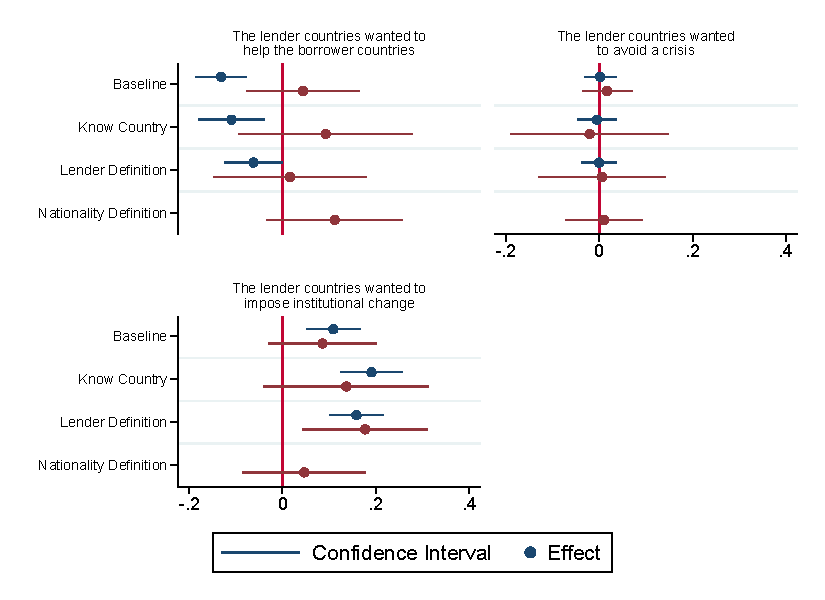
\includegraphics[scale=1.2]{belief_question2.pdf}
    \label{fig:my_label}
    \end{center}
    \tiny 
    \tablenotes{Participants were asked to assess the following statements:  Question 2.1: The lender countries wanted to help the borrowing countries Question 2.2: The lender countries wanted to help themselves avoid a crisis at home Question 2.3: The lender countries wanted to impose institutional change upon the borrower countries }
\end{figure}
\begin{figure}[h!]
    \begin{center}
     \caption{ Emotions of program countries (Beliefs) }
    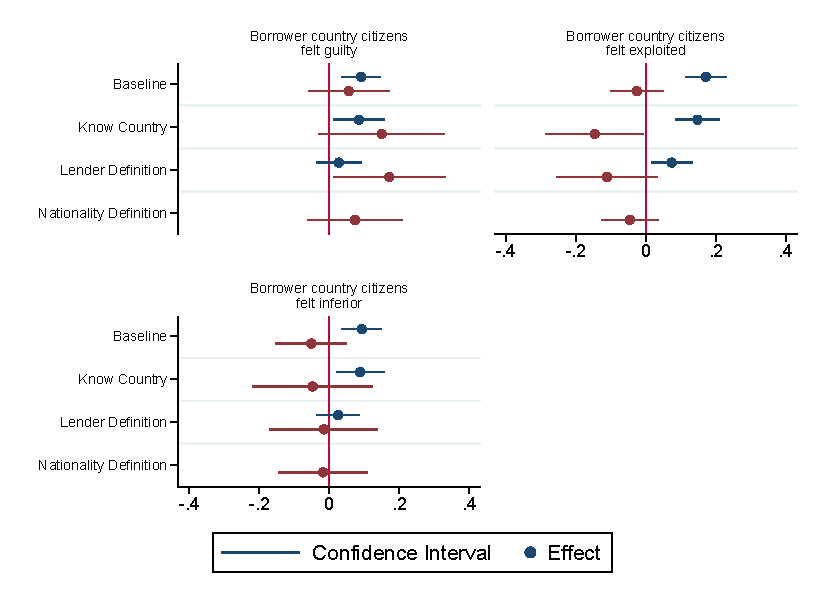
\includegraphics[scale=1.2]{belief_question51.pdf}
    \label{fig:my_label}
    \end{center}
    \tiny 
     \tablenotes{Question 5.1: The rescue experience made many citizens in the borrower countries feel guilty; Question 5.2: The rescue experience made many citizens in the borrower countries feel exploited; Question 5.3: The rescue experience made many citizens in the borrower countries feel inferior} 
\end{figure}
\begin{figure}[h!]
    \begin{center}
     \caption{ Emotions of non-program countries and repayment of outstanding debt (Beliefs)}
    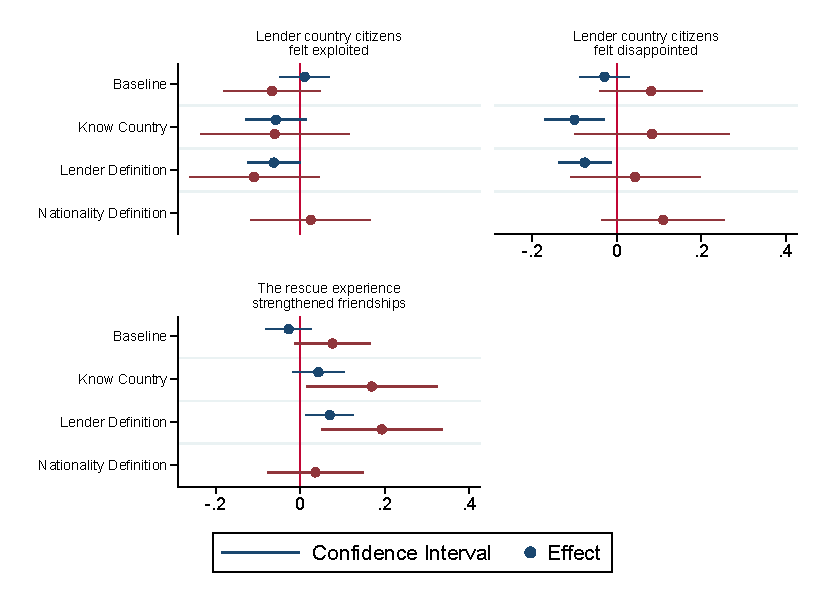
\includegraphics[scale=1.2]{belief_question52.pdf}
    \end{center}
    \tiny
     \tablenotes{Question 5.4: The rescue experience made many citizens in the lender countries feel exploited; Question 5.5 The rescue experience made many citizens in the lender countries feel disappointed Question 5.6: The rescue experience strengthened friendships between citizens Question 7: Greece will fully pay back it's debt}
\end{figure}
\begin{figure}[h!]
    \begin{center}
     \caption{Who initiated and benefited from the rescue program (Beliefs) }
    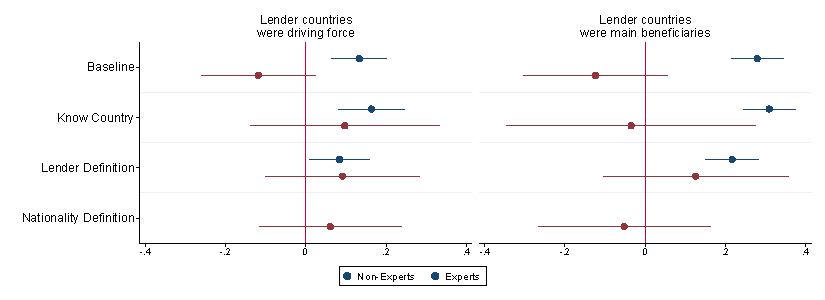
\includegraphics[scale=1.2]{belief_question34.pdf}
    \end{center}
    \tiny
    \tablenotes{Question 3: Who was the driving force behind signing the memorandum; Question 4: Who was the main beneficiary of the program; Question 7: Who primarily benefited from the loans to Greece}
\end{figure}
\begin{figure}[h!]
    \begin{center}
     \caption{Situation in Greece (Beliefs)}
    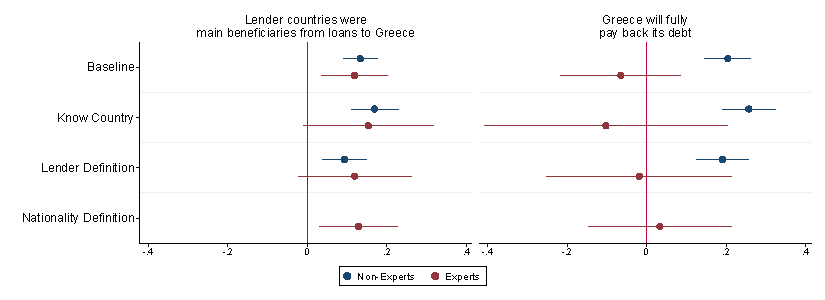
\includegraphics[scale=1.2]{belief_question67.pdf}
    \end{center}
    \tiny
    \tablenotes{Question 6: Who primarily benefited from the loans to Greece? ;  Question 7: Greece will fully pay back it's debt}
\end{figure}










